\section{Introducci\'on}
%\addcontentsline{toc}{section}{Introducci\'on}

En el presente trabajo intentaremos resolver mediante distintas t\'ecnics algor\'itmicas el problema de la \textit{k-Partici\'on de M\'inimo Peso} (\textbf{k-PMP}).

Primero es necesario introducir la idea de partici\'on de conjuntos. Una partici\'on de un conjunto A consta de varios de subconjuntos no vac\'ios de A disjuntos, tales que la uni\'on de todos ellos es A.  Es decir, sea $P = \{A_{i}: i ∈ I \}$, se cumple:
\begin{itemize}
\item Para cada $i \in I$, $A_{i} \subseteq A$ y $A_{i} \neq \emptyset$
\item Para cada par $i \neq j, A_{i} \cap A_{j} = \emptyset$
\item $\bigcup_{i \in I} A_{i} = A$
\end{itemize}
Adem\'as, una \textit{k-partici\'on}, es una partici\'on con $k$ subconjuntos.

Esta noci\'on se puede trasladar a grafos. Un grafo G se representa con dos conjuntos V y W tales que V, corresponde a los v\'ertices y W a las aristas, una partici\'on de G consiste en particionar el conjunto de v\'ertices V, bajo la definici\'on de partici\'on de conjuntos, por ejemplo, $G=(V,W)$ con $V=\{1,2,3\}$ es decir, el grafo con los v\'ertices 1 2 y 3, las posibles particiones de G son $\{\{1\},\{2,3\}\}, \{\{1,2\},\{3\}\}, \{\{1,3\},\{2\}\}, \{\{1\},\{2\},\{3\}\}$ y todo el conjunto $\{1,2,3\}$. Cabe aclarar que en el desarrollo del trabajo, tomamos al conjunto vac\'io como un posible subconjunto perteneciente a una  partici\'on, por ejemplo $\{1,2,3\},\{\}$ es v\'alida como partici\'on de G, por lo que la \'unica propiedad de la definici\'on de Partici\'on de conjuntos que no se cumple es la primera.

Al particionar un grafo, podemos identificar dos tipos de ejes. Las \textit{aristas intrapartici\'on} que son aquellas tal que ambos extremos pertenecen a un mismo subconjunto de una partici\'on o dicho formalmente, sea $V_{1},V_{2},...,V_{k}$ una partici\'on de $V$ una arista $uv \in W$ es intrapartici\'on si existe un $i \in \{1,...,k\}$, tal que $u, v \in V_{i}$. De la misma manera, podemos diferenciar las aristas que no corresponden a ninguna partici\'on como aquellas tales que sus extremos pertenecen a subconjuntos distintos.

Para ejemplificar el problema gr\'aficamente, la figura \textbf{Figura \ref{ejemplito2}} es una \textit{2-partici\'on} del grafo de la \textbf{Figura \ref{ejemplito1}}. Las aristas $(1,2)$ y $(3,4)$ no son intrapartici\'on ya que los v\'ertices de sus extremos quedaron en distintas particiones, mientras que las aristas $(1,3)$, $(3,5)$, $(5,6)$ y $(2,4)$ si lo son.


\begin{figure}[H]
	\begin{subfigure}{.5\textwidth}
		%\centering
		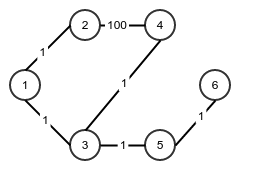
\includegraphics[scale=0.6]{intro/ejemplito1.png}
		\caption{Grafo original}
		\label{ejemplito1}
	\end{subfigure}
	\begin{subfigure}{.5\textwidth}
		\centering
		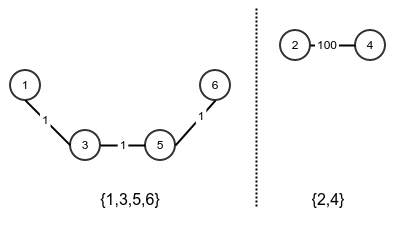
\includegraphics[scale=0.5]{intro/ejemplito2.png}
		\caption{Partici\'on}
		\label{ejemplito2}
	\end{subfigure}
\caption{}
\label{}
\end{figure}

Volviendo al problema \textbf{k-PMP}, dada una funci\'on de peso $\omega : E \rightarrow R+$, definida
sobre las aristas de G, el peso de una k-partici\'on es la suma de los pesos de las aristas intrapartici\'on, por lo que el objetivo es hallar la de m\'inimo peso con respecto a cualquier otra k-partici\'on. Por ejemplo en la \textbf{Figura \ref{ejemplito2}} la suma de las aristas intrapartici\'on es $103$ mientras que si particionamos dejando los extremos de la arista con peso 100 en distintas particiones como muestra la \textbf{Figura \ref{ejemplito3}} logramos un peso total de $4$ y m\'as a\'un, si particionamos como en la \textbf{Figura \ref{ejemplito4}} logramos un peso total de $2$.

\begin{figure}[H]
	\begin{subfigure}{.5\textwidth}
		%\centering
		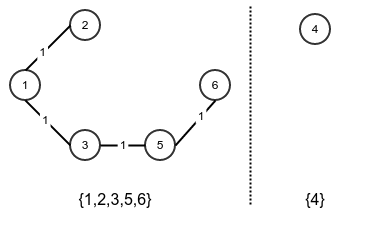
\includegraphics[scale=0.5]{intro/ejemplito3.png}
		\caption{Partici\'on con peso total 4}
		\label{ejemplito3}
	\end{subfigure}
	\begin{subfigure}{.5\textwidth}
		\centering
		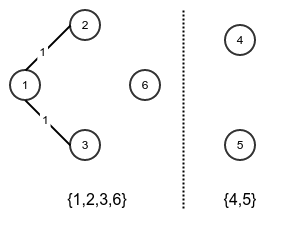
\includegraphics[scale=0.5]{intro/ejemplito4.png}
		\caption{Partici\'on con peso total 2}
		\label{ejemplito4}
	\end{subfigure}
\caption{}
\label{}
\end{figure}

Es importante notar que la partici\'on de la \textbf{Figura \ref{ejemplito4}} es una k-PMP, pero no es la \'unica, ya que existen otras como la $\{2,3,5,6\},\{4,1\}$ tambi\'en con peso $2$.

El problema \textit{k-Partici\'on de M\'inimo Peso} o \textit{Minimum K-Cut} (en Ingl\'es) es un problema \textbf{NP-Completo} \footnote{Garey M.R. and Johnson D.S., "Computers and intractability: a guide to the theory of NP- Completeness", W. Freeman and Co., 1979. (a),(c)} por lo que no se conoce un algoritmo polinomial que lo resuelva, es por esto que a lo largo del trabajo, vamos a dar una algoritmo basado en la t\'ecnica de \textbf{backtracking} para obtener una de las soluciones ''exactas´´ pero de gran complejidad computacional, para luego explorar la \textbf{Heur\'istica Golosa}, la \textbf{B\'usqueda Local} y por \'ultimo \textbf{GRASP}, que nos ayudaran a acercarnos a la soluci\'on lo m\'as posible con ordenes de complejidad m\'as bajos.